\section{PS3: Pythagorean Tree}\label{sec:ps3}

\subsection{Overview}\label{sec:ps3:overview} % A discussion of the assignment itself

This project creates a Pythagorean Tree from a given side length, size, and angle measure.
A Pythagorean Tree starts as a square, and generates two more squares (of possible different sizes depending on the given angle measure) in opposing directions.
Each new square will generate two new squares in the same manner as many times as the given recursion depth.

\subsection{End Product}\label{sec:ps3:accomplish} % What I accomplished and images/results

Below is the output.
This is the simplest version of the tree using a 45 degree angle.

\begin{figure}[h]
\centering
\begin{minipage}[b]{0.4\textwidth}
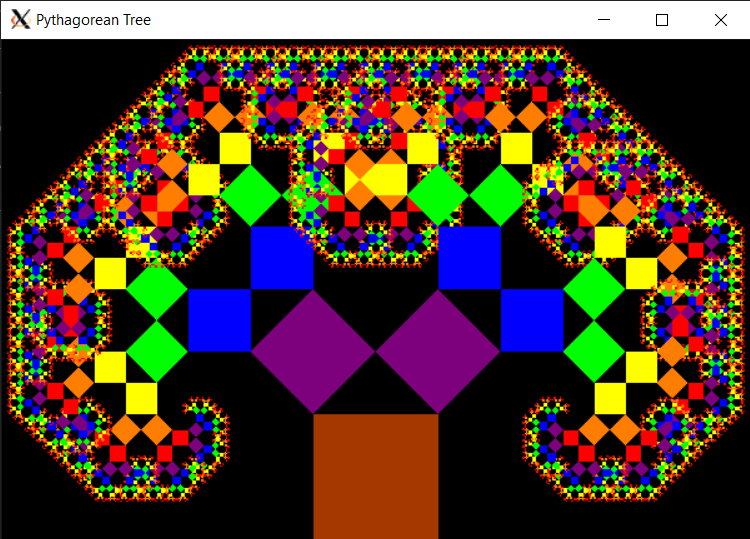
\includegraphics[width=\textwidth]{ps3-1_output}
\caption{Pythagorean Tree: 45 Degrees}
\end{minipage}
\end{figure}

\subsection{What I Already Knew}\label{sec:ps3:knew} % What was known prior to the assignment

I had SFML experience from past projects and basic manipulation fo rectangular shapes.
As for C++, I knew a how to create a basic tree and node class and use recursion within them.

\subsection{Design Decisions and Implementations}\label{sec:ps3:decisions} % Important decisions or implementations I made

I chose to make two classes, a Tree class and a Node class.
A tree object has a root Node which represents the starting square in this case.
Each Node is a rectangular sprite with the addition of a left and right node member to generate future squares.
The Tree calls upon a recursive 'grow' function which creates two children from a given parent Node with the correct new position, angle, size, etc.
This recursion loops for the given depth.

\bigskip
For extra credit, I added two things.
The first feature I added was color changing depening on the depth of the tree.
The starting color is always brown (like a stump) and then any following levels loop through the rainbow.
The second feature I added was the ability to chnage the angle of the new generated squares.
However, in doing so, a problem arose which is coverd in the challenges section.

\subsection{What I Learned}\label{sec:ps3:learned} % What I learned because of the assignment

I learned what a Pythagorean tree is and how it's made.
I learned more about SFML shapes and how translations effect them.

\subsection{Challenges}\label{sec:ps3:challenges} % Challenges along the way and any that went unresolved

I came across a few different challenges.
The first was setting the origin of every new object.
SFML API is pretty bad at documenting this, along with it being confusing in general, so it took me a while to get each new rotation/position correct.
The second, I was unable to fix, and was the problem resulting from doing the extra credit mentioned above which involves changing the angle of recursion.
With a changed angle the tree may no longer fully fit to the generated window.
I could not figure out a proper way to make a window that would prefectly fit any given generated tree to screen.

\newpage
\subsection{Codebase}\label{sec:ps3:code} % Code: Makefile, .cpp main, .hpp main, .cpp support, .hpp support, .cpp tests

\bigskip
\title{\large Makefile:}
\lstinputlisting{../ps3/Makefile}
\bigskip
\title{\large main.cpp:}
\lstinputlisting{../ps3/main.cpp}
\bigskip
\title{\large Sokoban.cpp:}
\lstinputlisting{../ps3/PTree.cpp}
\bigskip
\title{\large Sokoban.hpp:}
\lstinputlisting{../ps3/PTree.hpp}

\newpage
